\documentclass[a4paper, 11pt]{report}

% Venturer Camp 2023 Final Report & Evaluation preamble


% BASIC PAGE SETUP
\usepackage{geometry}
\geometry{
a4paper,
total={170mm,257mm},
left=20mm,
top=20mm,
}
\setlength\parindent{0pt} % get rid of the stupid indent

% set toc depth to only show chapters
\setcounter{tocdepth}{0}

% use section numbering for everything up too and including subsubsection
\setcounter{secnumdepth}{3}


% PACKAGES

\usepackage{tikz} % Required for drawing custom shapes
\usetikzlibrary{arrows, backgrounds, calc, fit, math, mindmap, positioning, shapes, shapes.geometric, tikzmark}

\usepackage{xcolor}

\usepackage{pgffor}

\usepackage{titlesec}
\usepackage[T1]{fontenc}
\usepackage[hidelinks]{hyperref}
\hypersetup{
pdftitle={Venturer Camp 2023 Final Report \& Evaluation},
pdfauthor={Thomas Boxall},
}

\usepackage{pgf-pie}

\usepackage{ragged2e}
\usepackage{float}
\usepackage{multicol}
\usepackage{multirow}
\usepackage{longtable}

\usepackage{appendix}
\usepackage{pdfpages}


\renewcommand{\arraystretch}{1.6} % make cells vertically bigger
\usepackage{colortbl}

% Headers and Footers

\usepackage{fancyhdr}
\pagestyle{fancy}
\fancyhf{}
\fancyhead[L]{Final Report \& Evaluation}
\fancyhead[R]{Venturer Camp 2023}
\fancyfoot[L]{\leftmark}
\fancyfoot[C]{}
\fancyfoot[R]{\thepage}
\renewcommand{\footrulewidth}{0.4pt}
\addtolength{\topmargin}{-1.59999pt}
\setlength{\headheight}{13.59999pt}

\raggedbottom
% Venturer Camp 2023 Final Report & Evaluation Preamble (Titles)

\newcommand{\drawhexagon}[5]{
    % #1 - text
    % #2 - position
    % #3 - size
    % #4 - rotation
    % #5 - options
    \node[rounded corners, inner sep=0, ultra thick, regular polygon, regular polygon sides=6, minimum size=#3, rotate=#4, #5] at (#2) {#1}
}

\newcommand{\drawtext}[5]{
    % #1 - text
    % #2 - position
    % #3 - height
    % #4 - rotation
    % #5 - options
    \node[left, bg, rounded corners, minimum width=\paperwidth, minimum height=#3, text width=\paperwidth, rotate=#4, #5] at (#2){#1}
}

\definecolor{accent}{HTML}{6d8f41}
\colorlet{fg}{black}
\colorlet{fgalt}{darkgray}
\colorlet{fgacc}{black}
\colorlet{bg}{white}
\colorlet{bgalt}{lightgray}
\colorlet{bgacc}{orange}
\colorlet{border}{black}
\colorlet{borderalt}{darkgray}
\colorlet{borderacc}{orange}


\titleformat{\chapter}[hang]{\Huge\bfseries}{\textcolor{accent}{\thechapter\hspace{0.75em}}\textcolor{accent}{|}\hspace{0.75em}}{0pt}{\Huge\bfseries}
\titleformat{\section}[hang]{\LARGE\bfseries}{\textcolor{accent}{\thesection\hspace{10pt}}\textcolor{accent}{}\hspace{0pt}}{0pt}{\LARGE\bfseries}
\titleformat{\subsection}[hang]{\Large\bfseries}{\textcolor{accent}{\thesubsection\hspace{10pt}}\textcolor{accent}{}\hspace{0pt}}{0pt}{\Large\bfseries}
\titleformat{\subsubsection}[hang]{\large\bfseries}{\textcolor{accent}{\thesubsubsection\hspace{10pt}}\textcolor{accent}{}\hspace{0pt}}{0pt}{\large\bfseries}

\titlespacing*{\chapter}{0pt}{0em}{2em}

\newcommand{\partTitlePage}{%
  \begin{tikzpicture}[remember picture,overlay]

    \pgfdeclarelayer{bg}    % declare background layer
    \pgfdeclarelayer{fg}    % declare background layer
    \pgfsetlayers{bg,main,fg}  % set the order of the layers (main is the standard layer)


    \fill[bg] (current page.south west) rectangle (current page.north east);


    \foreach \i in {0.5,...,20} {\drawhexagon{}{$(current page.north west)+(2.5,0)$}{\i cm}{0}{accent!60,draw};}


    \foreach \i in {21,...,2} {\drawhexagon{}{$(current page.south east)+(-0.2,-0.45)$}{\i cm}{0}{accent!85,draw};}


    \begin{pgfonlayer}{fg}
    \drawtext{\raggedleft \LARGE\partname{} \thepart}{$(current page.center)+(9.5, -5.5)$}{3cm}{0}{text=fg,align=right};
    \end{pgfonlayer}

    \end{tikzpicture}%
}

% Customize the part page
\usepackage{titlesec}
\titleformat{\part}[display]
  {\Huge\bfseries\filcenter}
  {\partname{}\thepart}
  {0pt}
  {\partTitlePage\Huge\bfseries}


% redefine \chapter so it uses pagestyle=fancy
\makeatletter
\renewcommand\chapter{\if@openright\cleardoublepage\else\clearpage\fi
\thispagestyle{fancy}%
\global\@topnum\z@
\@afterindentfalse
\secdef\@chapter\@schapter}
\makeatother


\newcommand{\makeDocumentTitle}{%
\begin{titlepage}
    % \pagestyle{empty}
    % \newgeometry{left=0cm,top=0cm,right=0cm,bottom=0cm}

    \begin{tikzpicture}[remember picture,overlay]

    %%%%%%%%%%%%%%%%%%%% Layers %%%%%%%%%%%%%%%%%%%%%%%%
    \pgfdeclarelayer{bg}    % declare background layer
    \pgfdeclarelayer{fg}    % declare background layer
    \pgfsetlayers{bg,main,fg}  % set the order of the layers (main is the standard layer)

    %%%%%%%%%%%%%%%%%%%% Background %%%%%%%%%%%%%%%%%%%%%%%%
    \fill[bg] (current page.south west) rectangle (current page.north east);

    %%%%%%%%%%%%%%%%%%%% Background Polygon %%%%%%%%%%%%%%%%%%%%

    % top left
    \foreach \i in {0.5,...,20} {\drawhexagon{}{$(current page.north west)+(2.5,0)$}{\i cm}{0}{accent!60,draw};}

    % bottom left
    \foreach \i in {2.5,...,22} {\drawhexagon{}{$(current page.west)+(2.5,-5)$}{\i cm}{0}{accent!60,draw};}

    % center right
    \foreach \i in {0.5,...,22} {\drawhexagon{}{$(current page.north east)+(0,-9.5)$}{\i cm}{0}{accent!90,draw};}

    % bottom right
    \foreach \i in {21,...,2} {\drawhexagon{}{$(current page.south east)+(-0.2,-0.45)$}{\i cm}{0}{accent!85,draw};}

    %%%%%%%%%%%%%%%%%%%% Title + Subtitle %%%%%%%%%%%%%%%%%%%%
    \drawtext{\Huge{\textbf{Final Report \& Evaluation}}\\\Large\textsc{Venturer Camp 2023}}{$(current page.center)+(3.2,-3.2)$}{3cm}{-60}{text=fg,align=right};

    %%%%%%%%%%%%%%%%%%%% Author Name %%%%%%%%%%%%%%%%%%%%
    \begin{pgfonlayer}{fg}
    \drawtext{\Large\textsc{Woodcraft Folk}\\\Large\textsc{January 2023}}{$(current page.east)+(-0.5,-5.2)$}{2cm}{0}{text=fg,anchor=east,align=right};
    \end{pgfonlayer}

    %%%%%%%%%%%%%%%%%%%% Year %%%%%%%%%%%%%%%%%%%%
    \drawhexagon{\Large }{$(current page.west)+(2.5,-5)$}{2.5 cm}{0}{accent!60,draw,text=fg};

    \end{tikzpicture}
    \restoregeometry
\end{titlepage}
}

\begin{document}
\makeDocumentTitle

\tableofcontents


\part{Background \& Introduction}
    \chapter{Coordinator's Introduction}

Welcome to the Venturer Camp 2023 Final Report \& Evaluation.\\

For the most part, this document has been co-authored by the entire Venturer Camp team, with the Coordinator and Woodcraft Folk Events Assistant producing the first draft. This section, however, has solely been written by me - Thomas Boxall, Camp Coordinator.\\

To coordinate such a big Woodcraft Event was a great privilege. I grew up as a young person in Woodcraft and after seeing the impact the Covid Pandemic has had on the young people of today, I'm honoured to be able to say that I've changed these young people's lives by giving them a space where they can be themselves, have fun, forget the pressures of the outside world and take part in workshops centred around Woodcraft Folk's values.\\

However, saying that the year which we made Venturer Camp happen in was an easy one - would be a lie. Just saying it was a difficult one would also be a lie. The year from August 2022 to August 2023 was probably one of the most challenging years I've had in my life, due to a number of things - my role in coordinating Venturer Camp being one of them. \\

Woodcraft Folk is really great at empowering young people to do things, look at me - I was 19 while coordinating this thing. However, it's not good at supporting them to do big scary things like this. To say the year I was coordinating Venturer Camp was tough on my mental health would be an understatement. I'm extremely grateful for those around me who were able to catch me when I fell, both in and out of Woodcraft. They were the reason I was able to coordinate the camp. You know who you are - thank you for that.\\

Saying this, Woodcraft is good at catching people. From speaking to teams while writing this evaluation - I wasn't the only one to struggle with the work. Many of the teams had more and more work piled onto them, or individual members within teams who initially agreed to take on a small role ended up being instrumental in the success of that team's work. Through all the ever-increasing workloads, teams pulled it off. They more than pulled it off, they did it so well that we didn't notice how well they did it - the ultimate sign of success when it all goes smoothly.\\

Why Woodcrafter's have to fall before they can be supported is something that we need to consider, as an organisation. We cannot leave this untouched if we want to be a sustainable organisation which supports its members to try new things.\\

Pulling an event like Venturer Camp 2023 together in 365 days is by no means an easy feat. The countless hours of dedication from Volunteers up and down the country were the reason 450 people were able to be together in a field for 7 days and mostly have a good time. The majority of the work required to pull this event together fell to a relatively small group of active volunteers. Whilst it may seem from the outside that we had a substantial number of volunteers involved in the project, many of these weren't able to commit to a large role leaving a small core team to do most of the work. Throughout this report, you'll hear about different teams' struggles with capacity and workload management. Every core team member should be commended for how well they managed, how well they coped with the ever-increasing workload and how well they rose to the challenge of pulling off a Venturer Camp in a year. Don't ever try and do it in a year again, it's a silly idea.\\

I'm extremely proud of everyone who had a part to play in the success of Venturer Camp, all those who contributed countless hours making meticulous spreadsheets; those who contacted suppliers and chased to get the cheapest and best meatballs they could; those who cleaned the toilets and showers; and especially those who turned up, tried something new and had fun. We wouldn't have done this without you - thank you for that.\\

I want to leave you to enjoy the rest of this evaluation with a quote: ``we do this because we love Woodcraft''.\\

Blue skies,\\

Thomas Boxall\\

Venturer Camp 2023 Coordinator\\
<thomas@woodcraft.org.uk>

    \chapter{Introduction to the Evaluation}
This Final Report \& Evaluation of Venturer Camp 2023 has been primarily compiled by Thomas Boxall, Venturer Camp 2023 Coordinator (Volunteer), and Millie Burgh, Woodcraft Folk Events Assistant (Staff).\\

Every effort has been made to ensure that this report is as accurate and representative of all teams as possible. However, there may be times where this was not possible. All data referenced throughout this evaluation is available on request. Please contact the Camp Coordinator should you have any questions or wish to seek clarification on anything.

\section{Methods Used}
Opinions and Thoughts from the wider coordination team were gathered through a series of interviews conducted by the Camp Coordinator and Events Assistant. \\

Feedback from participants was gathered during the event itself through a Workshop run on a village level. Not all villages submitted notes from their workshop, so participant evaluations may not be representative of all participants on site. \\

All Volunteers involved in the project were invited to complete a Google Forms questionnaire after camp where they could give feedback. As expected with a survey like this, not all volunteers have responded and those who have responded would fall at either end of the spectrum, either having lots of good things to say or lots of bad things. Conversations had with volunteers throughout the event have been included.
\begin{figure}[h]
    \centering
    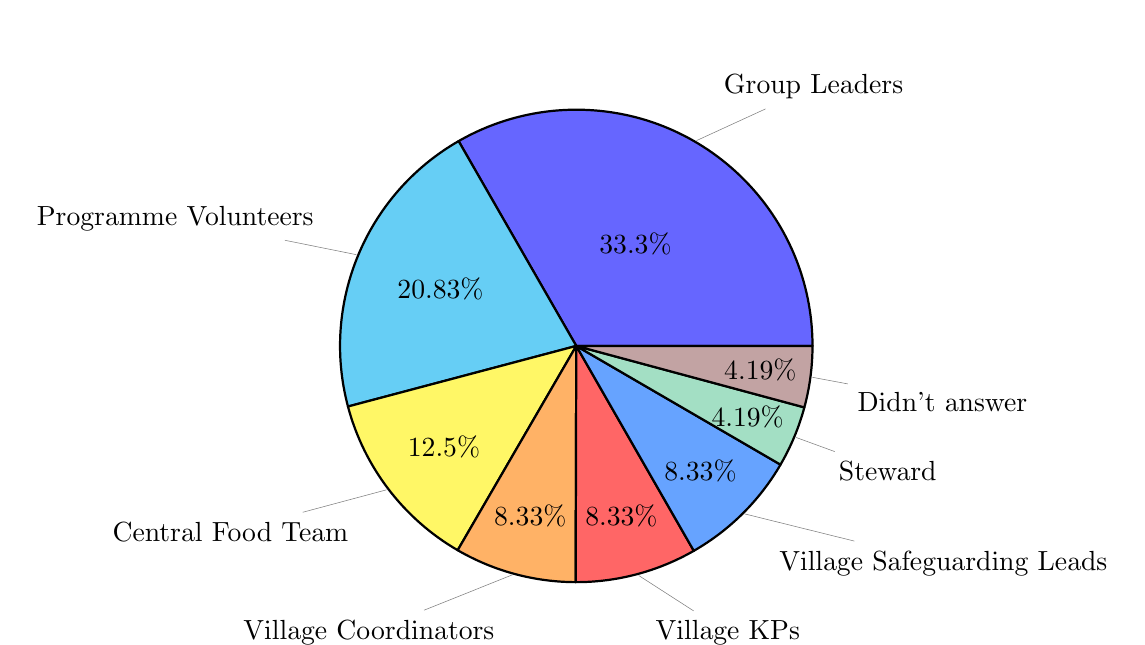
\begin{tikzpicture}
        \pie[text=pin]{33.3/Group Leaders,
        20.83/Programme Volunteers,
        12.5/Central Food Team,
        8.33/Village Coordinators,
        8.33/Village KPs,
        8.33/Village Safeguarding Leads,
        4.19/Steward,
        4.19/Didn't answer
        }
    \end{tikzpicture}
    \caption{Respondents to the Google Form Questionnaire}
    
\end{figure}

\section{Why Such A Long Evaluation?}
To put it simply, we should be evaluating our projects like this properly. Big camps are such a fundamental part of Woodcraft Folk's operations and with the organisation nearing its 100th birthday, you'd think we've got pretty good at getting lots of Woodcrafters in a field together having a good time. This is only mostly true, however.\\

This report aims to cover what we did, how we did it, and why we did it. As well as if it worked, how people found it and what we'd do differently in the future. \\

In all reality, there's going to be very few people who read the entirety of this document from cover to cover. However, people taking on roles at future large camps should be encouraged to read the sections relevant to them. 

\section{Photo Credits}
Photos have been used throughout this report, the captions include the initials of the photogropher, see below for names of those photographers:
\begin{description}
    \item[AB] Alex Baird
    \item[IC] Isabel Cleveland
    \item[RS] Ralph Sleigh
    \item[TB] Thomas Boxall
\end{description}

\section{Contact Information of Those Mentioned}
Due to this report being made available to the public on the internet, contact information of most people involved in this project has been redacted. The exceptions to this are Woodcraft Folk members of staff and the Camp Coordinator.\\

To obtain the contact information of anyone mentioned in the report - please contact Thomas Boxall, Camp Coordinator via \href{mailto:thomas@woodcraft.org.uk}{thomas@woodcraft.org.uk}

    \chapter{Introduction To The Project}
\section{Idea Conceptualisation}
Venturer Camp normally happens every 3 years, as a national camp for Venturers (the 13-15 year olds in Woodcraft Folk). 16 year olds are also normally allowed to come as participants if they haven't experienced a Venturer Camp before.\\

Typically a volunteer team provides infrastructure for the central area, a central menu, some central programme in the form of workshops in the daytime and some evening entertainment, and put groups in `villages' where they will eat, sleep and do clan. Group leaders bring their young people and organise their village including infrastructure, clans and activities.\\

For a long time Venturer Camp happened at Drum Hill Scout Campsite in Derbyshire, but in 2019 for the first time we held it at Biblins, Woodcraft Folk's own site in the Wye Valley. \\

There were two key things we wanted to do differently from past Venturer Camps this time round. Firstly, due to Common Ground being postponed 2 years because of COVID, this camp was to be 4 years after the Venturer Camp before opposed to the usual 3. For this reason, we expanded the participant age range to 17, to ensure as many young people as possible get to experience a Venturer Camp. \\

Another focus of this camp was volunteer support. Building on Common Ground, where for the first time there was a volunteer wellbeing role on the camp team, we wanted to ensure all volunteers (both central and village volunteers) were well supported on camp. We didn't manage to do as much as we wanted in this respect as we were only able to recruit one person for the volunteer support team who could support ahead of camp and on site, but the majority of the central team were able to get a day off with planning and support, which definitely hasn't been the norm in the past.

\section{Planning Timeline}
The decision was made in summer 2022 to hold a Venturer Camp the following August (we go into more detail why in the `What Dates' section). Because of this we only had a year to plan the camp when preparation usually starts around 2 years in advance. While most things don't happen until the final year, this extra year is pretty key when it comes to recruiting volunteers, building trust and care among the team and getting started with some key decisions and actions. Much of what could have been improved this camp came down to not having enough volunteers or volunteers not feeling confident/part of a team, which may not have been fully rectified by having an extra year but this almost certainly would have helped.\\

We have shown a Venturer Camp can be planned in a year, but not without either having a full team from early on or seriously overworking some members of the team. Therefore we would recommend always beginning plans 2 years in advance where possible.

\part{Event Decisions}
    \chapter{Finding A Suitable Site}
For Venturer Camp 2023, the decision of what site to use was perhaps easier than in previous years. The accelerated timeline for the project meant that we would have had great difficulty finding a suitable site for Venturer Camp (thinking about infrastructure requirements on the site, transport links to the site, location in the country, etc).\\

Ultimately, we used Biblins Youth Campsite, which is owned by Forestry England and leased to Woodcraft Folk. Using a site which is managed by Woodcraft Folk, gives us greater flexibility and a level of quality assurance which would be unknown for other sites which we haven't worked with before.\\

From the feedback about the previous Venturer Camp's choice of site, also held at Biblins in 2019, you wouldn't have thought that we would use the site again. A large proportion of the campers commented that they were a very long distance from their village to the central area. These complaints were mostly from those camping on pitch 1 where they had to walk to Pitch 6 and 7 for the central programme. Since 2019, Biblins has undergone renovation works to relocate Camp Koodoo (its permanent camp) from Pitch 5 to adjacent to Pitch 1a. This resulted in us being able to centralise our central area onto pitches 4 and 5. We received little-to-no complaints about walking distance from villages to the central area, other than from those volunteers who would be in the central area up until meal times who would have to return to their village, collect food and then get straight back to the central area to finish programme delivery. This issue was quickly rectified, however, by the volunteers getting food delivered from their village to the central area. \\

For many months, the Coordination team had very little contact with the Biblins Staff Team; however, as camp approached, we had more contact with the team to gain information about the workings of the site, infrastructure on site and get copies of their policies and procedures which we would potentially need to implement while on site.\\

During the event itself, the Coordinator and Project Staff Team worked closely with the Biblins Staff Team, which enabled clear communication about issues and matters which arrose on site such as The Spill, access to the Bunkhouse Basement Storage and Adventurous activities, including a major change of plans to the Canoeing. \\

Having direct contact with the Biblins Staff Team proved invaluable and made the event considerably easier to organise.

    \chapter{Deciding on Dates}
\section{2023 v 2024}
As part of the project kick off, dates for the event had to be decided. However, before we could decide exactly which dates to host the camp on, we had to decide on a year first. This was a complex debate, with many people weighing in on the decision, ranging from Trustees to venturer group leaders to venturers themselves.\\

The ultimate decision was made that the camp should be hosted in 2023. We came to this decision based on the preference of Venturer Leaders and Venturers themselves to host the camp in 2023. This data was captured through a survey which ran for a few weeks in September 2022, the results of which can be seen in Table \ref*{tab:year-survey-results}

\begin{table}[h]
    \centering
    {\RaggedRight
    \begin{tabular}{p{0.2\textwidth} p{0.2\textwidth} p{0.2\textwidth} p{0.2\textwidth}}
    \textbf{} & \textbf{2023} & \textbf{No Preference} & \textbf{2024}\\
    \hline
    \hline
    Leaders & 56\% & 11\% & 33\% \\
    \hline
    Venturers & 67\% & 11\% & 22\% \\
    \hline
    \end{tabular}
    } % end of rr     
    \caption{Results of Year Survey}
    \label{tab:year-survey-results}
\end{table}

The survey also provided space where the respondents could share any thoughts, feelings, or suggestions. The responses to this varied were varied, some of the responses are shown below:
\begin{itemize}
    \item ``I think another national camp would not be supported. We need to have district summer camps to get young people back into camping. We struggled like lots of districts getting pioneers to common ground without a summer camp next year we will struggle to get children back into summer camps after the disruption of covid''
    \item ``Some venturers want a `proper camp before they are too old.' Adults want a break in 2024 before 100 camp''
    \item ``It would be good to have a date to be able to add to the calendar and to try and not book family holidays at the same time.''
    \item ``Personally, I think sooner is best as delaying by another year will inevitably mean some venturers won't get the chance to go. The venturers were mixed in responses, with a small majority favouring 2023 but others saying either or 2024. If it is next summer, please avoid clashing with the international camp in Finland (24-31 July 2023). Also, a question from our venturers is whether DFs who missed their chance to go to VCamp because of covid would be able to attend? Thanks''
    \item ``I have a venturer and a DF happy to help''
\end{itemize}

At the time of making the decision, we did not have a fully fleshed out team. There were significant gaps of knowledge and experience in the following teams:
\begin{itemize}
    \item Food
    \item Site Services \& Production
    \item Programme
    \item Communications
    \item Access \& Inclusion
    \item Event Administration (however we expected this role to be done by the Woodcraft Folk Events Assistant, so weren't worried about recruitment)
\end{itemize}
The lack of some of these teams presented a challenge for project initiation as once we had decided on 2023, they couldn't influence it and as such this deterred people from joining the team.\\ 

A volunteer close to the coordinator who supported him a lot said ``it's very dangerous when we organise the camp in a very short timeframe with a big dependence on one individual as it puts them in a vulnerable position and goes against our aims and principles. Empowering people to take on roles they've not done before is good but they need support in place. We need to ask questions about how they are supported.'' It was these questions around support networks which were answered when they were asked; when the coordinator was struggling, not pre-emptively. Pulling off a Venturer Camp in such a short amount of time, with such a limited capacity team. was not an easy thing to do (yes we did have a large number of people on it but many were limited in their capacity to be involved due to other commitments). Woodcraft Folk put too much pressure on the Camp Coordinator who was also juggling many other things, see introduction, which should never happen again.

\section{Which Dates In 2023}
The decision of what dates we wanted to host the camp on came down to four things:
\begin{enumerate}
    \item The dates which Biblins was available
    \item Festivals \& other attractive-to-young-people summer events
    \item School Term Dates (taking into account the early return of Scottish Schools)
    \item Finnish International Camp Dates
\end{enumerate}

At first, we chose the dates Monday 7 August to Monday 15 August. These dates were put to the Coordination team who decided that we would rather start and end on a weekend to reduce the amount of annual leave adult volunteers would have to take.\\

After some deliberation, we decided on Saturday 5 August to Saturday 12 August. These dates did't clash with any major festivals, were early enough that Scottish Young People would have a few days between camp finishing and their term dates starting, there were a few days between the Finland International Camp finishing and Venturer Camp starting, however the whole of the campsite was not available for all of these dates. There was a group booked onto pitch 1a for the night of Saturday 5 August. The decision was made that we wouldn't need that part of the site for the first night and so could press on with publishing the dates and working out the rest of the timeline.

\section{Group on Pitch 1a}
We took a gamble with the group on pitch 1a being a nice group who wouldn't mind 450 people descending onto the site. For the most part, the gamble paid off - the group were lovely and were interested in what we were doing. However, at first they weren't keen on the numbers of people who were camping to the West side of The Spill. We gave them a wide berth after they indicated this and had no further complaints or comments from them. 
    \chapter{Booking Timelines}
Once we had decided on dates for the camp, we could begin to work backwards designing timelines to suit. We settled on the public timeline shown in Table \ref{tab:booking-public-timeline}

\begin{table}[h]
    \centering
    {\RaggedRight
    \begin{tabular}{p{0.3\textwidth} p{0.5\textwidth}}
    \textbf{Date} & \textbf{Event}\\
    \hline
    \hline
    27 January 2023 & Bookings Open\\
    \hline
    12 April 2023 & Early Bird Booking Deadline\\
    \hline
    26 May 2023 & Final Booking Deadline\\
    \hline
    \end{tabular}
    } % end of rr     
    \caption{Public Booking Timeline}
    \label{tab:booking-public-timeline}
\end{table}

As we were designing the booking timeline, we made the decision to not close bookings. We believed that if we were to fully close bookings then we would be at risk of people turning up to camp who hadn't booked and would want to book on the door, or worse - they wouldn't tell the camp coordination team they had arrived which would complicate number based operations, such as food distribution or village size. We made a conscious decision to brand the 26 May 2023 deadline as the ``Final Booking Deadline'' in hope that we would deter people from booking late, and for the most part, we did.\\

We also had a second timeline, this was created and was published in the Payment Policy for Individuals and Groups, however it wasn't pushed onto people so they may not have known the late bookings were an option. One group reported that they treated the Early Bird Booking Deadline as their internal final deadline and another reported that they would accept bookings right up to the camp starting as long as the young person paid what they owed. 
\begin{table}[h]
    \centering
    {\RaggedRight
    \begin{tabular}{p{0.3\textwidth} p{0.5\textwidth}}
    \textbf{Date} & \textbf{Event}\\
    \hline
    \hline
    27 January 2023 & Bookings Open\\
    \hline
    12 April 2023 & Early Bird Booking Deadline\\
    \hline
    26 May 2023 & Final Booking Deadline\\
    \hline
    10 June 2023 & Booking Content Deadline\\
    & Refund Request Deadline (ad-hoc)\\
    \hline
    22 July 2023 & Late Booking Deadline\\
    \hline
    12 August 2023 & Very Late \& On-The-Door Booking Deadline\\
    \hline
    \end{tabular}
    } % end of rr     
    \caption{Internal Booking Timeline}
    \label{tab:booking-internal-timeline}
\end{table}

The refund deadline was added in an ad-hoc manner. This was due to the number of people wanting refunds for individuals coming up to the final booking deadline. The refund deadline was written into the payment policy and a second version was published on 24 May 2023.\\

Ultimately, not closing bookings proved valuable as a number of additional volunteers were recruited at DF camp to come and support the MEST-UP provision. These people paid the highest amount to come, the very late booking price, which supported us to hit our booking income target.

    \chapter{Who Do We Want To Come, Who Came?}

\section{Expanded Age Ranges}
Venturer Camps are traditionally held every three years. This cycle was disrupted by holding Common Ground International Camp in 2022, which was displaced from 2020 due to the Covid Pandemic. Not being able to hold a Venturer Camp in 2022, meant that there is one year's worth of Venturers who would have missed out on their Venturer Camp experience. For this reason, we decided to expand the age ranges of Venturer Camp 2023. The decision was made to include 16 and 17 year olds as Venturers. This would mean a small number of people who attended the 2019 camp as a participant would also be able to attend the 2023 camp as a participant.
\begin{figure}[h]
    \centering
    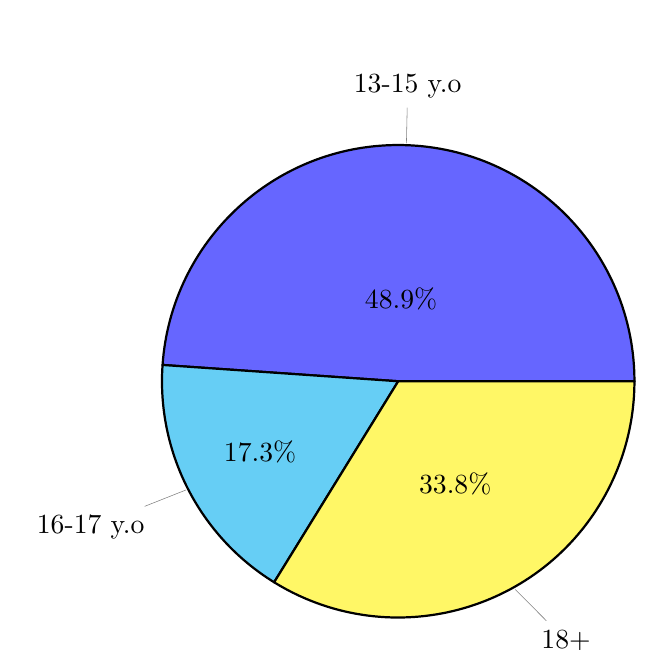
\begin{tikzpicture}
        \pie[text=pin]{48.9/13-15 y.o,
        17.3/16-17 y.o,
        33.8/18+
        }
    \end{tikzpicture}
    \caption{Booked attendees by age}
\end{figure}

By expanding the age ranges, we enabled more young people to participate in Venturer Camp 2023. We also enabled those 16 and 17 year olds who may never have experienced Woodcraft Folk outside their district or Common Ground, which was very structured, to have a looser structured Woodcraft Folk experience. The hope was that this would support them to transition to DFs, enabling them to grow their movement (the pandemic resulted in many DFs falling out of the movement). Figure \ref{fig:distribution-of-attendees} shows how some DFs were able to take on Volunteering roles as under-18 volunteers.
\begin{figure}[ht]
    \centering
    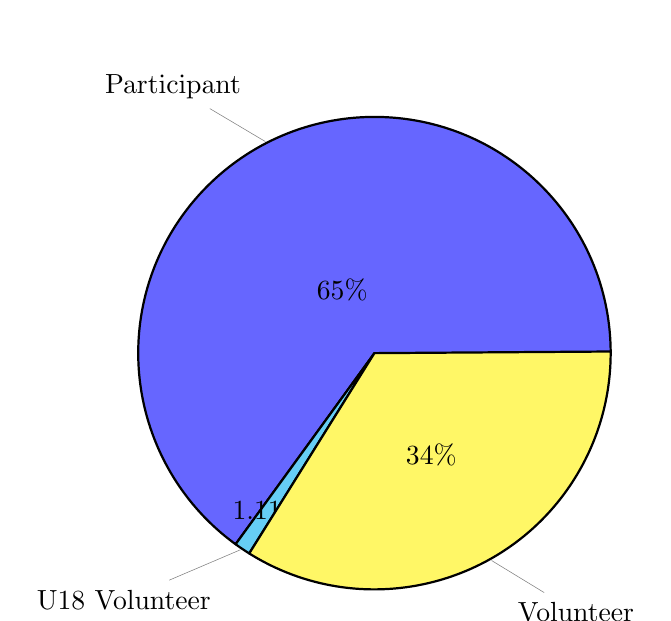
\begin{tikzpicture}
        \pie[text=pin]{65/Participant,
        1.11/U18 Volunteer,
        34/Volunteer
        }
    \end{tikzpicture}
    \label{fig:distribution-of-attendees}
    \caption{Distribution of Attendees}
\end{figure}

\section{International Delegations}
In Autumn 2022 we were also hoping that we would be able to support a number of international delegations to attend. We discussed a number of models through which we could facilitate this with a very small coordination team. The majority favoured being that a group or district would be responsible for all aspects of supporting an international delegation.\\

In Spring 2023, the general enquiries inbox was contacted about the possibility of hosting a group from an English Language school situated in Spain. However, due to the Woodcraft knowledge barrier and the implied expectation that we (the central coordination team) would be responsible for supporting this group to attend, the decision was made to decline this request. At this time, the coordination team was stretched very thinly, with many people taking on more than what they'd expected to be doing in the run up to the event.\\

We were, unfortunately, unable to host any international delegations at Venturer Camp 2023. 

\section{Centrally Organised Equipment}
During the conceptualisation of Venturer Camp 2023, we decided that to reduce burdens on Villages - we would centrally organise the equipment which was being assigned to Villages. This concept, what worked well and what didn't work about it will be explored in the Site Services \& Production Team's section - there are very mixed views about this!

    \chapter{Pricing}
After developing the booking timeline and deciding about the expanded age ranges, we were able to decide on pricing for the camp.\\

Woodcraft Folk is committed to working to reduce barriers towards Volunteering. One such barrier, Venturer Camp presented a perfect test ground for - is the financial commitment to come to a camp. This resulted in us having the following pricing structure.

\begin{table}[h]
    \centering
    {\RaggedRight
    \begin{tabular}{p{0.2\textwidth} p{0.2\textwidth} p{0.2\textwidth} p{0.3\textwidth}}
    \textbf{Before} & \textbf{Age Bracket} & \textbf{Whole Camp} & \textbf{1 night}\\
    \hline
    \hline
    \multirow{2}{*}{26 May 2023} & Under 18 & \pounds150 & \pounds21.50\\
    \cline{2-4}
    & 18 and over & \pounds50 & \pounds7.50\\
    \hline
    \multirow{2}{*}{22 July 2023} & Under 18 & \pounds225 & \pounds32.25\\
    \cline{2-4}
    & 18 and over & \pounds75 & \pounds11.25\\
    \hline
    \multirow{2}{*}{12 August 2023} & Under 18 & \pounds300 & \pounds43\\
    \cline{2-4}
    & 18 and over & \pounds100 & \pounds15\\
    \hline
    \end{tabular}
    } % end of rr     
    \caption{Pricing Structure based on 1-person figures}
\end{table}
We made the decision that all those attending the camp who are aged 18 and over would be attending as a volunteer, and as such we would recognise their contribution by charging them a third of the participant cost. 

\section{Under-18 Volunteer Priced Places}
Due to the enlarged age ranges for Venturer Camp 2023, we also wanted to ensure those who could technically come as participants had the opportunity to volunteer without paying the (higher) participant price.\\

This desire led to the creation of the Under 18 Volunteer Price Scheme whereby a young person aged 16 or 17 could apply for a volunteer priced place if they were at the camp primarily as a volunteer. The scheme required a few things of the young person before the price reduction could be allocated: 
\begin{enumerate}
    \item have begun the process of obtaining a Enhanced DBS (or membership of the PVG scheme if based in Scotland);
    \item be registered as a member of Woodcraft Folk and have paid their membership fee;
    \item have submitted references (this will normally have been done as part of becoming a member of Woodcraft Folk); and 
    \item have spoken to the relevant team leader about the role and a volunteer role description has been produced (this should be included with the application).
\end{enumerate}
This scheme was widely publicised, and despite this - we only had approximately 5 people take part in it. The roles they took on ranged from stewarding to centre coordinator to cafe \& special diets kitchen assistant.\\

There were a number of young people who had paid the participant price who attended to volunteer. These young people coordinated a centre as a group. They made the decision to pay the participant price as they also engaged in some other programme. For future events, it might be worth having an intermediary pricing point for those young people who are volunteering some of the time and also participating at other times. 

    \chapter{International Volunteers}
After Brexit, organisations in the UK are no longer eligible to participate in the European Solidarity Corps (ESC) programme run by the European Commission. Common Ground (2022 International Camp) was supported by a 15-strong team of ESC volunteers and as such, it was hoped that Venturer Camp 2023 would also be able to be supported by a number of international volunteers as those at Common Ground proved extremely valuable to the team.\\

Woodcraft Folk worked with a UK-based charity called Concordia to manage the recruitment of volunteers. A further evaluation of how this worked, what went well and what didn't work can be found in the Concordia chapter.

    \chapter{Venturer Committee's Involvement}
At the time of project kick-off for this event - there was no functioning Venturer Committee. This was due to the pandemic and the fact that all the current members had `aged-out'. This led to there being very little involvement in the planning process from Venturer aged people. It was an unfortunate loss to not have young people's voices on the planning committee. We had hoped to overcome this shortfall with a scheme called the \textit{Village People}

In September 2022, a meeting was held between key individuals where it was discussed about using Venturer Camp as a chance to re-form Venturer Committee. Due to a combination of factors, including lack of capacity in progressing with re-forming Venturer Committee, nothing happened with this until camp itself started.

On Camp, an individual planned and held Venturer Committee elections with the support of previous Facilitators. The elections held at the event were a great success and all roles on Venturer Committee were able to be filled. This individual also held other roles of responsibility on camp, and as such they had a very busy time. For future events, it would be recommended that an individual with no other commitments takes on the Venturer Committee Elections Facilitation role.

\section{Village People}
The Village People was a scheme designed to introduce the voice of the participants and the people who knew the participants the best into the planning of Venturer Camp 2023. In Autumn 2022, we invited all Venturer Leaders to apply to join the group. We then selected a representative sample, ensuring all types \& sizes of groups were represented.\\

The scheme unfortunately died out quite quickly due to extremely low response rates to opinion-gathering forms which went out. It would be lovely to see a scheme like this work at a future large Woodcraft Camp. 

\part{Event Administrations \& Communications}
    \chapter{Bookings}
\section{Booking System}
After discussions between the Camp Coordinator and Woodcraft Folk Chief Executive where different booking system options were reviewed, it was agreed to use Ralph Sleigh's custom system which had been first used at Venturer Camp 2019, then Common Ground 2022. Ralph and the Camp Coordinator had initial conversations about what features the booking system would require as Ralph had started re-writing the booking system to use different, more cost effective, technology.\\

During Autumn 2022, the Food and Special Diets teams were consulted about what data they wished to collect from those booking in. As the focus on special diets was new to Woodcraft Camps, a larger amount of data was captured about each individual booked on. Through using the custom booking system, the implementation of this was exactly as we wished, while using an off-the-shelf system we may not have been able to collect and view this data in the same way.\\

During January 2023, the booking system was tested with the core team. These tests enabled the workflow of approving bookings, the mechanics of booking and ensuring that the wording used in the system was clear. Also during this period, the Booking Handbook was written.\\

The decision was made to require ``applications to book'' before enabling people to book. This decision was made mostly by the fact that Common Ground used this feature. In reflection, it was the right decision to use as it enabled us to ensure people booked in a way that was convenient to us. Rather than individuals booking, we had larger groups booking and we had the say to stop individuals if needed where there was already a group booking for their group. This also enabled us to ensure there were no bookings from people unknown to Woodcraft, but we either received no or very few requests of this nature.\\

Throughout the use of the booking system, a number of bugs and issues arose with it. Ralph responded quickly to all of these, deploying a fix usually within 12 hours of the issue being reported. Ralph was also able to implement features which improved the usability of the system, for example, messaging manager messages to the Coordination Team Discord server which prevented the need to use the emails the system also sent.\\

Overall, the use of a booking system which was developed ``In house'' gave us greater flexibility, greater options and overall a much easier experience than that of an off the shelf system. \\

The booking system allowed users to be able to be assigned backend access to view some or all of the data entered by users. To ensure volunteers who were being given this access had some basic understanding of GDPR, a Data Protection Declaration was created which all backend users of the booking system were expected to sign before being granted access. This worked and while Woodcraft Folk is not providing basic GDPR training for its volunteers, is something which should be repeated for future events. The transcript of the declaration can be found in the Appendix.\\

One thing that wasn't so great about Ralph's system is that it couldn't automatically match up who has / doesn't have membership. Or at least we thought it couldn't. When we discussed this at one point Ralph said there was something he could try to rectify this, which is definitely worth exploring for future events which use this system. 

\section{Bookings Administration}
After the bookings opened - Thomas and Millie processed most of the administration around bookings. This involved things such as: managing applications to book, reviewing bookings to locate any access needs.\\

Before bookings opened - there were conversations around how we want people to book. The decision was taken to try to get people to book as groups, with the general principle of one booking per group; with central adult volunteers booking separately.
This system worked, mostly. There was one case in particular where a region decided to come together and due to the disconnected nature of the young people attending - they took the decision for all the parents to book their children on. Unfortunately, they decided to start making their booking on the date of the early booking deadline. This led to the booking applications being accepted.\\

With having the booking deadlines at midnight, this meant that the responsibility of being on standby to approve the booking applications which come in after the members of staff had finished for the day fell to a volunteer, which for this event fell to the Camp Coordinator. For future events, the booking system needs to be able to specify the time of a booking deadline so that it can be set for a more sociable hour! \\

The booking system generates a unique booking reference for each booking. This then means that when the money is transferred to the Woodcraft Folk Bank Account, we should be able to match up the payment to the booking. This works reasonably well, so far as people used the references and we were able to match up payments. The difficulties experienced with this system came from the structures of the Woodcraft Folk Finance Administration Systems, see below for a more detailed analysis of this. 

\section{Early Booking Deadline}
A decision was taken that the incentive for booking by the early-bird deadline was to receive a free limited edition t-shirt. This decision, whilst good in theory, creates a large financial overhead - where each t-shirt costs more than the financial discount would have been. Once this fact was discovered, it was agreed that we would expect people to have booked and paid their deposit by the Early Bird Booking Deadline to receive a free t-shirt.\\

The communications around the requirements for payment before the t-shirts were given out was not the best due to a number of factors. Primarily, it was down to time pressures that all locations promoting the early bird deadline weren't updated to reflect the payment requirement. The requirement to pay was communicated through the Payment Policy and through social media content leading up to the deadline.\\

Unfortunately, some groups didn't receive the message about the payment requirements. These caused tensions where group leaders had promised their young people free t-shirts and there were no free t-shirts for them as they had not paid by the deadline. These tensions were rectified by selling the group leaders t-shirts `at cost', rather than at the standard camp rate. Whilst not a perfect solution, it was accepted. \\

For those who did pay deposits \& book in advance of the deadline: a Google Form was used to gather the size requirements, which influenced the numbers of garments in each size we ordered. \\

It would not be recommended to do a free t-shirt as the reward for Early Bird bookings in the future. This is due to the complex administration requirements, and the difficulties experienced with advertising the offer

\begin{figure}[ht]
    \centering
    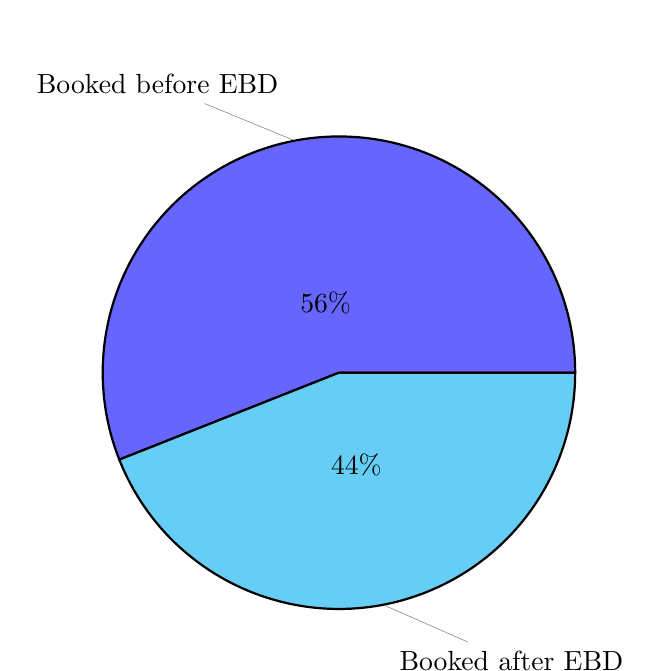
\begin{tikzpicture}
        \pie[text=pin]{56/Booked before EBD,
        44/Booked after EBD
        }
    \end{tikzpicture}
    \caption{Attendees booked before / after Early Bird Deadline (EBD)}
    
\end{figure}
    \chapter{Finance}
The finances for Venturer Camp 2023 were overseen by the Head of Resources at Woodcraft Folk with assistance and knowledge given from the Venturer Camp Treasurer and Coordinator. The decision to manage the finances like this came about from not having anyone in the treasurer post at the start of the project so the Coordinator and HoR began managing the finances themselves, then once a treasurer was appointed this felt like the simplest option. \\

The management of finances through the Woodcraft Folk systems had a number of benefits and drawbacks. The most notable benefit was that it was all dealt with for us (``us'' being the Core Team), with trained professionals managing the day to day running of the finance. The Treasurer was able to support by approving expenses and invoice payments as well as doing the first level of chasing for payments, later levels of chasing were done by the HoR.\\

One of the significant drawbacks of using the very established Woodcraft Folk finance system is that it is already set up very firmly. The Venturer Camp team's budget lines didn't match the central monitoring system, and this made our lives much more difficult when reviewing payments into and out of the account in order to monitor how much was being spent in each category. This was further exacerbated by the fact that the finance monitoring tools (a series of Google Sheets) were set up such that they required a great level of understanding to be able to read them. This resulted in large amounts of confusion amongst those people who had to read them and understand them. \\

Another significant drawback of using the Woodcraft Folk finance system was that quite often transactions were ``mis-coded'' within the system. This resulted in transactions erroneously appearing on the monitoring spreadsheet, or not appearing altogether - leading us to believe we hadn't spent as much as we in fact had. 

\section{Budget}
The first budget for Venturer Camp 2023 was drawn up by Woodcraft's Chief Executive using figures from Venturer Camp 2019 and Common Ground International Camp 2022 to influence expected expenditure for 2023. Throughout the project, minor alterations were made to the budget, mostly to reflect the change in expected income due to fundraising income being lower than initially expected.\\

Due to the above mentioned issues with income and expenditure coding within the Woodcraft Folk finance systems, and the fact that they do not line up with our budget lines - we do not have a final breakdown of expected vs actual for our budget.\\

Shown below is the Venturer Camp 2023 budget, compared to the Venturer Camp 2019 actual expenditure. 



\end{document}


%table template
\begin{table}[h]
    \centering
    {\RaggedRight
    \begin{tabular}{p{0.2\textwidth} p{0.2\textwidth} p{0.2\textwidth} p{0.3\textwidth}}
    \textbf{Name} & \textbf{Predecessor} & \textbf{Successor} & \textbf{Examples}\\
    \hline
    \hline
    Linear & unique & unique & stack, queue\\
    \hline
    Hierarchical & unique & many & family tree, management structure\\
    \hline
    Graph & many & many & railway map, social network\\
    \hline
    Set Structure & no & no & DSALG class\\
    \hline
    \end{tabular}
    } % end of rr     
    \caption{Classifications of Data Structures}
\end{table}